\hypertarget{activity-dates-and-times}{%
\section{Activity Dates and Times}\label{activity-dates-and-times}}

Question: What are the dates and timestamps of when contributor
activities occur?

\hypertarget{description}{%
\subsection{Description}\label{description}}

Individuals engage in activities in open source projects at various
times of the day. This metric is aimed at determining the dates and
times of when individual activities were completed. The data can be used
to probabilistically estimate where on earth contributions come from in
cases where the time zone is not UTC.

\hypertarget{objectives}{%
\subsection{Objectives}\label{objectives}}

\begin{itemize}
\tightlist
\item
  Improve transparency for employers about when organizational employees
  are engaging with open source projects
\item
  Improve transparency for open source project and community managers as
  to when activity is occurring
\end{itemize}

\hypertarget{implementation}{%
\subsection{Implementation}\label{implementation}}

\hypertarget{filters}{%
\subsubsection{Filters}\label{filters}}

\begin{itemize}
\tightlist
\item
  Individual by Organization
\item
  Aggregation of time by UTC time

  \begin{itemize}
  \tightlist
  \item
    Can show what times across the globe contributions are made; when
    the project is most active.
  \end{itemize}
\item
  Aggregation of time by local time

  \begin{itemize}
  \tightlist
  \item
    Can show what times of day in their local times they contribute.
    Conclusions about the If contributions are more during working
    hours, or if contributions are more during evening hours.
  \end{itemize}
\item
  Repository ID
\item
  Segment of a community, (e.g., GrimoireLab has more EU time zones
  activity and Augur more US time zones activity)
\end{itemize}

\hypertarget{visualizations}{%
\subsubsection{Visualizations}\label{visualizations}}

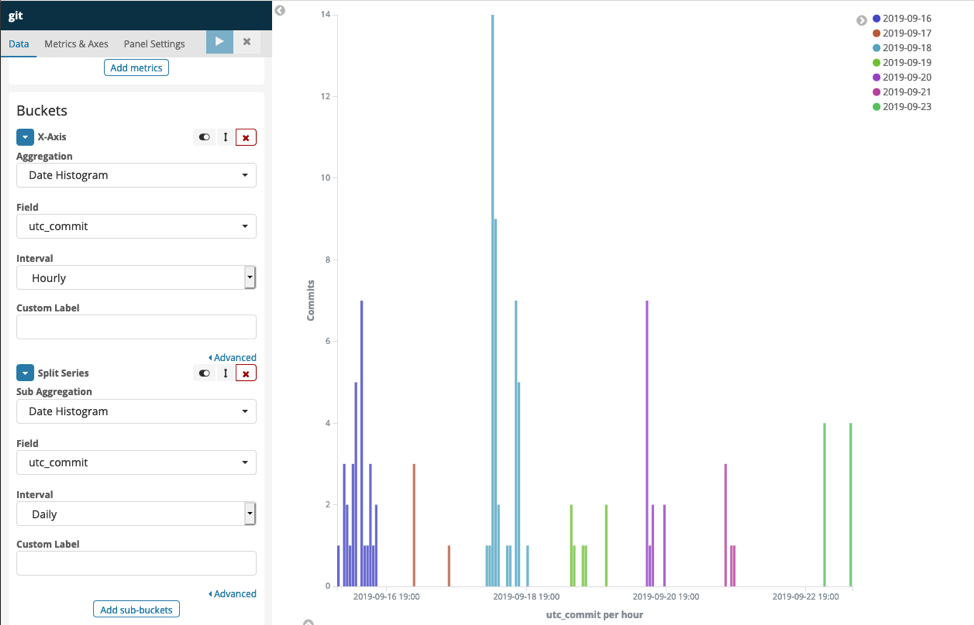
\includegraphics{images/activity-dates-and-times_1.png}
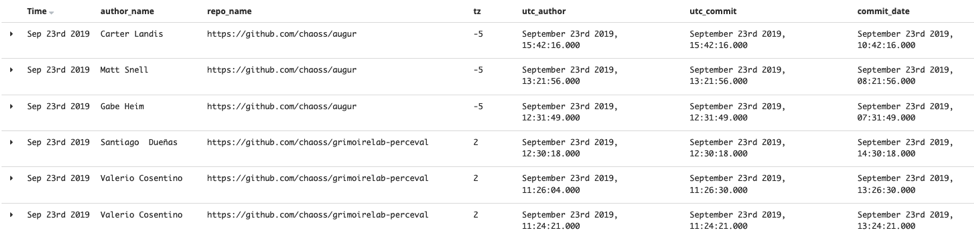
\includegraphics{images/activity-dates-and-times_2.png}
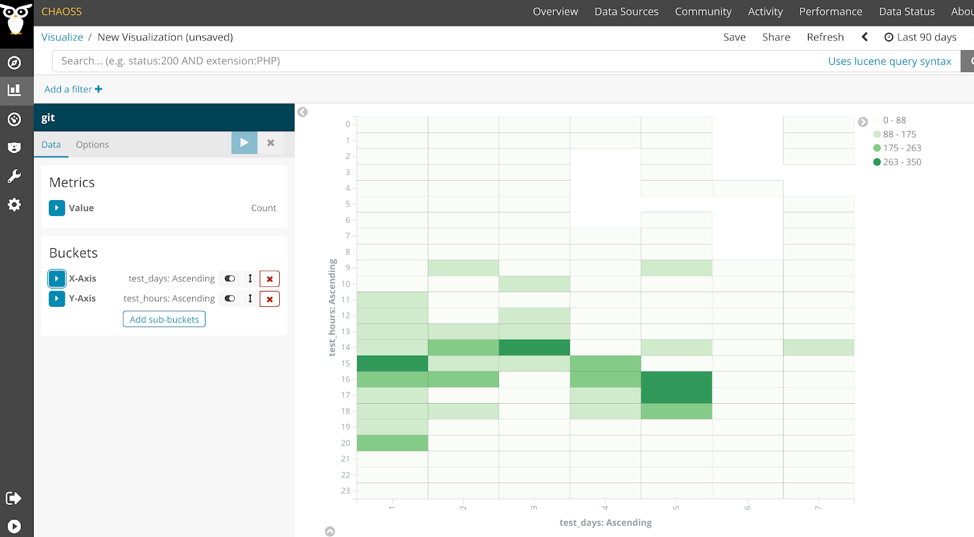
\includegraphics{images/activity-dates-and-times_3.png}
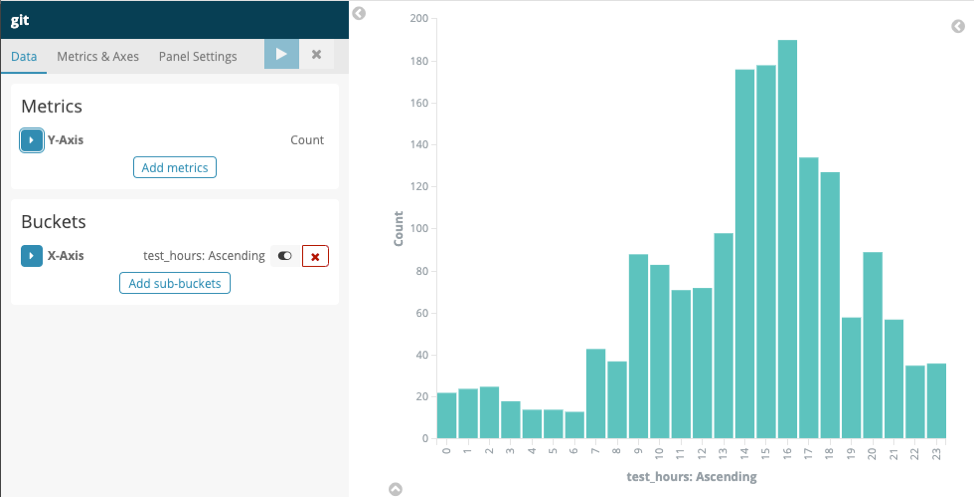
\includegraphics{images/activity-dates-and-times_4.png}

\hypertarget{tools-providing-metric}{%
\subsubsection{Tools Providing Metric}\label{tools-providing-metric}}

\href{https://chaoss.github.io/grimoirelab/}{GrimoireLab}

\href{https://docs.augur.net/\#dates-timestamps}{Augur Date/Timestamps}

\hypertarget{references}{%
\subsection{References}\label{references}}

\href{https://en.wikipedia.org/wiki/Coordinated_Universal_Time}{Coordinated
Universal Time}
